% =====================================================================
%  Capítulo 3 — Arquitetura do sistema
% =====================================================================
\chapter{Arquitetura do sistema}
\label{cap:arquitetura}
\rubricaJustificativa

\begin{orientacao}
Arquitetura é o conjunto de decisões que custam caro para desfazer.
Este capítulo não descreve o que a equipe montou --- isso é o
Capítulo~\ref{cap:implementacao} --- e sim \emph{por que} montou assim,
e o que foi descartado no caminho. As caixas \DP{n} são o instrumento
principal da fatia de 25\,\% da rubrica reservada à justificativa
técnica. Uma decisão sem alternativa descartada não é decisão: é a
primeira coisa que ocorreu à equipe.
\end{orientacao}

\section{Visão em camadas}

\begin{orientacao}
Localize o sistema nas quatro camadas vistas em 17/08: percepção, rede,
processamento e aplicação. Diga, para cada camada, o que existe no
projeto \emph{neste ciclo} --- na \rotuloAP\ é normal que a camada de
rede seja um cabo USB e um monitor serial, e dizer isso com todas as
letras é melhor que fingir que existe uma nuvem. Marque também onde o
processamento acontece (borda, névoa ou nuvem) e por quê.
\end{orientacao}

Na AP1, o sistema ocupava apenas a percepção e o processamento na borda,
e a camada de rede era só o cabo USB e o monitor serial de bancada.
Neste ciclo, as quatro camadas do modelo visto em 17/08 passam a ter
algo dentro. A camada de \textbf{percepção} continua sendo o nó
ESP32~+~DHT22: lê temperatura e umidade, filtra o dado e decide
localmente se ele está dentro da faixa configurada. O
\textbf{processamento} da decisão de alarme continua inteiramente na
borda, pela mesma razão da AP1: o alarme não pode depender da rede, que
agora existe mas pode cair (\DP{5}). A camada de \textbf{rede} passa a
ser o WiFi do ESP32 até o roteador e, dali, MQTT sobre TLS (porta 8883)
até o \emph{broker} público \texttt{broker.hivemq.com}
(Seção~\ref{sec:tecnologia}). O armazenamento fica com o gravador, um
assinante MQTT em Python que roda no notebook de João Pedro Saleh,
na tomada, e grava o conjunto de dados em CSV
(Seção~\ref{sec:caminho}). Na camada de \textbf{aplicação}, o que existe
neste ciclo é o próprio terminal do gravador, que imprime cada mensagem
ao chegar, o MQTT Explorer para ver os tópicos ao vivo e, depois da
coleta, o \texttt{qualidade.py} e o gráfico da série
(\texttt{grafico.py}).

Na campanha, o nó da placa rodou o \emph{firmware} do Lab~03 com o
DHT22 (branch \texttt{lab3}), e não o \emph{firmware} da AP1: a leitura
é única, sem mediana nem EMA, e não há alarme local. A decisão de alarme
na borda (\DP{5}) continua valendo para o produto, mas \textbf{não rodou
na campanha}; juntar as duas versões é a primeira tarefa do próximo
ciclo.

Esse é o caminho da campanha, com um nó falando direto com o roteador. A
arquitetura do produto, desenhada em paralelo pela equipe, tem um degrau
a mais: vários \textbf{nós de
borda} (um por sala ou câmara) falam com um \textbf{nó central} por
unidade, e só o nó central fala com a internet, enviando as leituras em
lote, por HTTPS e com uma chave de API própria, a um servidor com API
FastAPI e banco PostgreSQL, que alimenta o painel web. O servidor já
existe e, neste ciclo, recebeu as \num{1213} leituras reais da campanha
por uma ponte que faz o papel do nó central (Seção~\ref{sec:ponte},
\CT{16}); o \emph{firmware} de nó do produto ainda não tem rádio. Entre
os nós de borda e o nó central, a arquitetura usa \textbf{LoRa}, como
previa a arquitetura original e como aponta a matriz de decisão
(Seção~\ref{sec:tecnologia}): o nó de borda pode ficar dentro de um
freezer ou numa câmara fria, onde \SI{2,4}{\giga\hertz} atravessa mal. O
módulo LoRa comprado pela equipe não chegou a tempo para este ciclo; no
lugar dele, a equipe testou os dois rádios do próprio ESP32, ESP-NOW e
BLE. O ESP-NOW foi bem até \SI{8}{\metre} com uma parede, mas não há
garantia de que repita esse resultado através da parede metálica de um
freezer, e o BLE perdeu o enlace antes
(Seções~\ref{sec:espnow-bancada} e~\ref{sec:tecnologia}). A escolha do
hardware do nó central (outro ESP32 com um módulo LoRa ou um
Raspberry Pi) continua em aberto. O alarme continua na borda nas duas
versões. Arquiteturas de baixo custo com vários nós ESP32, cada um com a
própria lógica de controle e o próprio atuador e trocando dados por
publicação e assinatura, já foram validadas em automação residencial
\cite{perezayala2025esp32}; o TermoLOG segue o mesmo princípio, com a
diferença de que um nó central concentra a saída para a internet. A Figura~\ref{fig:arquitetura} mostra as duas versões lado a
lado, camada por camada.

\begin{orientacao}
Substitua pela figura da arquitetura. Um diagrama de blocos feito à mão
e fotografado é aceitável; um diagrama que não mostra por onde o dado
passa, não. Salve o arquivo em \texttt{figuras/} e ajuste o nome abaixo.
\end{orientacao}

% AP2: figura refeita com a camada de rede (gerada por
% figuras/gera_figuras_ap2.py). A da AP1 continua em
% figuras/arquiteturaCamadas.png.
\begin{figure}[H]
\centering
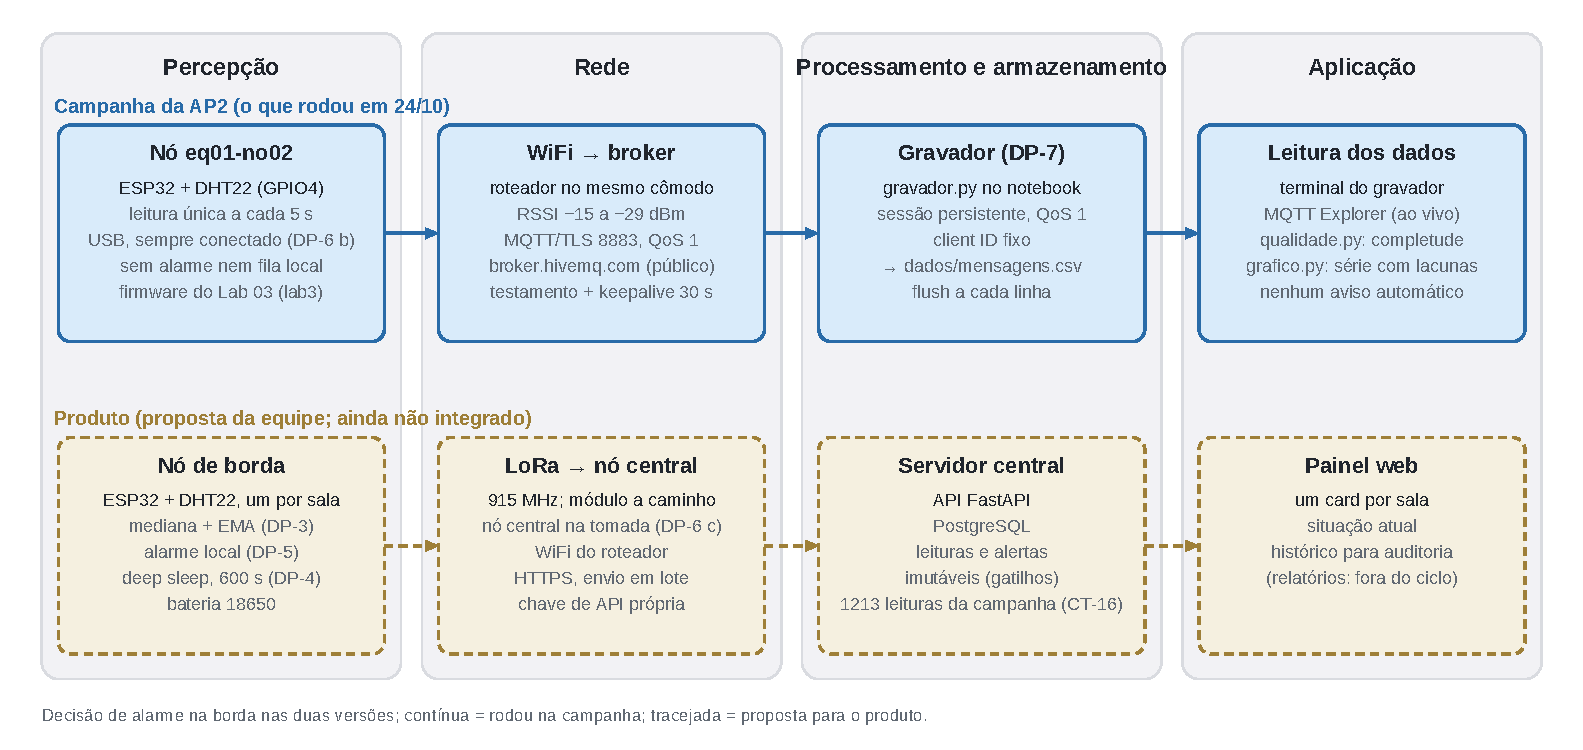
\includegraphics[width=\textwidth]{figuras/arquitetura-ap2.pdf}
\caption{Arquitetura do sistema em camadas: em cima, o que rodou na
  campanha da AP2; embaixo, a arquitetura proposta para o produto}
\label{fig:arquitetura}
\fonte{Elaborada pela equipe.}
\end{figure}

\section{Componentes e decisões de projeto}
\label{sec:componentes}

\begin{orientacao}
Uma caixa por decisão que a equipe realmente tomou. Três a cinco caixas
em um relatório de \rotuloAP\ é a faixa esperada. Candidatas típicas:
escolha do sensor, escolha do atuador, onde fica o limiar de decisão,
como o sistema se comporta sem energia, e por que o dado é (ou não é)
gravado localmente.
\end{orientacao}

\begin{decisao}{Escolha do sensor de temperatura e umidade}
\alternativas{DS18B20 (só temperatura, exigiria um segundo sensor e um
  segundo pino para a umidade), BME280 (mede temperatura, umidade e
  pressão via I\textsuperscript{2}C, custo mais alto) e sensor
  industrial calibrado do tipo usado pelos concorrentes comerciais
  (Novus, Testo), com incerteza de laboratório mas custo por unidade
  de milhares de reais.}
\criterio{O ambiente exige as duas grandezas no mesmo ponto de
  medição (\RF{01}); o custo por sala precisa caber em \RNF{03}
  ($\leq$ R\$\,150,00); o componente precisa estar disponível para a
  equipe.}
\escolha{DHT22 / AM2302.}
\evidencia{O DHT22 mede temperatura e umidade relativa em um único
  chip, por R\$\,39,90 (Tabela~\ref{tab:bom}), contra um DS18B20 que resolveria
  apenas a temperatura e ainda exigiria um sensor de umidade à parte
  --- mais um componente, mais um pino, mais um ponto de falha. A
  incerteza declarada em \folhadedados{} ($\pm$\SI{0.5}{\celsius} e
  $\pm 2$--\SI{5}{\percent} de UR) é suficiente para sinalizar desvio
  de faixa, que é o que \RF{02}/\RF{03} exigem --- o projeto não
  precisa da precisão de um datalogger de laboratório. Com o ESP32
  (R\$\,39,00), o nó completo fica em R\$\,105,20 com protoboard,
  alarme e componentes de reserva (Tabela~\ref{tab:bom}), cerca de
  trinta vezes mais barato que os
  concorrentes comerciais levantados na Cap.~\ref{cap:problema}, que
  usam sensores industriais calibrados justamente para justificar o
  preço.}
\consequencia{O conversor A/D já é do sensor (Aula~06): não existe
  sinal bruto para calibrar, e o erro sistemático de fábrica não é
  corrigível por \emph{software} --- apenas declarado junto de cada
  leitura (Seção~\ref{sec:sinal}). O sensor também impõe um intervalo
  mínimo de \SI{2}{\second} entre leituras, o que limita quantas
  amostras cabem em um ciclo de filtragem (Seção~\ref{sec:sinal}).}
\end{decisao}

\begin{decisao}{Tensão de alimentação do DHT22}
\alternativas{Alimentar em 5\,V com conversor de nível lógico
  bidirecional no fio de dado; alimentar em 5\,V com divisor resistivo
  no fio de dado; alimentar diretamente em 3V3.}
\criterio{O ESP32 não tolera 5\,V em seus pinos GPIO --- a tensão
  máxima admitida fica em torno de \SI{3.6}{\volt} (Aula~03) --- e o
  dano por sobretensão costuma ser silencioso e cumulativo, não
  imediato.}
\escolha{Alimentar o DHT22 em 3V3.}
\evidencia{O DHT22 aceita de 3,3 a 5,5\,V (\folhadedados{}). Alimentado
  em 3V3, o nível alto do seu pino de dado também sai em
  $\approx$\SI{3.3}{\volt}, compatível diretamente com o GPIO do
  ESP32.}
\consequencia{Elimina a necessidade de conversor de nível ou divisor
  resistivo no fio de dado, ao custo de exigir um cabo mais curto até
  o sensor caso a instalação futura precise de mais distância --- se
  isso ocorrer, a alimentação em 5\,V com conversor de nível volta a
  ser a opção recomendada, não o divisor resistivo, que arredonda as
  bordas do sinal em barramentos mais rápidos.}
\end{decisao}

\begin{decisao}{Filtragem da leitura do sensor}
\alternativas{Usar a leitura única do DHT22 sem filtro; aplicar apenas
  uma média aritmética das últimas N leituras; aplicar mediana de N
  amostras por ciclo combinada a uma média exponencial (EMA) entre
  ciclos.}
\criterio{Robustez a uma leitura isolada inválida (falha de
  \emph{timing} ou ruído elétrico no fio de dado, e não ruído de
  sinal analógico, já que o conversor é do próprio sensor --- Aula~06)
  sem herdar o atraso de uma janela longa, dado o custo em tempo
  acordado (e portanto em energia) de cada amostra extra.}
\escolha{Mediana de 5 amostras por ciclo de leitura, seguida de EMA
  entre ciclos de sono ($\alpha = 0{,}30$).}
\evidencia{A mediana descarta com eficiência um valor isolado
  incoerente sem distorcer o resultado inteiro, ao contrário de uma
  média aritmética simples. O custo é declarado: como o próprio
  sensor exige um intervalo mínimo de \SI{2}{\second} entre leituras,
  5 amostras custam cerca de \SI{8,4}{\second} de nó acordado por
  ciclo. Quando menos de 3 das 5 amostras são válidas, o
  \emph{firmware} declara falha em vez de calcular uma mediana pouco
  confiável.}
\consequencia{Cada ciclo de leitura consome mais tempo acordado do que
  uma leitura única resolveria, o que entra diretamente no orçamento
  de energia (Seção~\ref{sec:energia}).}
\end{decisao}

\begin{decisao}{Gerenciamento de energia entre leituras}
\alternativas{\emph{Modem-sleep}, \emph{light-sleep} e \emph{deep
  sleep} (as três estratégias de economia de energia do ESP32
  discutidas na Aula~08).}
\criterio{Autonomia de bateria nos nós de borda, que segundo a
  Cap.~\ref{cap:requisitos} podem ficar em pontos sem tomada
  acessível (dentro de um freezer, por exemplo), onde a troca
  frequente de bateria é indesejável e a fiação até a rede elétrica
  nem sempre é viável.}
\escolha{Deep sleep, com única fonte de despertar por temporizador.}
\evidencia{É o único dos três modos em que quase todo o chip desliga,
  o que dá autonomia de dias a meses em vez de horas --- ao custo de
  que a RAM comum se perde a cada ciclo, e o programa recomeça do
  \texttt{setup()} a cada despertar (Aula~08).}
\consequencia{Todo o \emph{firmware} precisou ser reorganizado para
  caber dentro do \texttt{setup()} (Seção~\ref{sec:firmware}), e as
  poucas variáveis que precisam sobreviver ao sono --- contador de
  despertares, médias exponenciais, contagem de falhas consecutivas
  --- são declaradas em memória RTC (\texttt{RTC\_DATA\_ATTR}), a
  única que atravessa o \emph{deep sleep}.}
\end{decisao}

\begin{decisao}{Onde processar os dados agregados do sistema}
\alternativas{Processamento na borda (o próprio nó ESP32 calcula
  histórico, tendências e regras mais complexas) versus processamento
  em um servidor central, para o qual os nós enviariam apenas as
  leituras.}
\criterio{Custo energético por ciclo em um nó alimentado por bateria
  (Apêndice~\ref{ap:energia}), já que qualquer processamento adicional
  mantém a CPU acordada por mais tempo em vez de voltar ao \emph{deep
  sleep}.}
\escolha{Processamento em servidor central; o nó de borda permanece
  responsável apenas pela leitura, pela filtragem local (mediana +
  média exponencial) e pela decisão simples de alarme dentro da faixa
  configurada.}
\evidencia{O estado de \emph{deep sleep} já responde por cerca de
  68\,\% do consumo diário estimado mesmo sendo o de menor corrente
  instantânea (Apêndice~\ref{ap:energia}); qualquer tempo extra de CPU
  acordada para processamento teria impacto direto e desproporcional
  na autonomia da bateria.}
\consequencia{A arquitetura distribuída (nó~+~servidor central) foi o
  objeto da AP2. O nó continua decidindo só o alarme, mas a decisão
  não evitou retrabalho: o nó da AP1, em \emph{deep sleep}, não foi
  integrado à rede neste ciclo, e unir a leitura filtrada e o alarme
  ao \emph{firmware} de comunicação é a primeira tarefa do próximo
  (\DP{6}, Cap.~\ref{cap:conclusao}).}
\end{decisao}

\subsection*{Decisões do Módulo 2}
\phantomsection
\addcontentsline{toc}{subsection}{Decisões do Módulo 2}

\begin{orientacao}
Novo na AP2. A escolha da tecnologia de comunicação fica na
Seção~\ref{sec:tecnologia}; aqui entram as decisões de
\emph{arquitetura} que mudaram por causa dela. A caixa abaixo registra
o conflito mais evidente entre a AP1 e a AP2: o nó da AP1 dorme em
\emph{deep sleep} (\DP{4}), e o \emph{keepalive} e o testamento do MQTT
pressupõem uma conexão que permanece aberta. Preencham com a decisão
que a equipe tomou de fato.
\end{orientacao}

\begin{decisao}{Deep sleep da AP1 \emph{versus} conexão permanente com o \emph{broker}}
\alternativas{(a) Manter o \emph{deep sleep} da AP1: a cada despertar,
  associar à rede, conectar ao \emph{broker}, publicar e desconectar;
  (b) abandonar o \emph{deep sleep} e manter o nó conectado, em
  \emph{modem-sleep} ou \emph{light-sleep}, com \emph{keepalive} e
  testamento ativos; (c) separar os papéis: o nó de borda mantém o
  \emph{deep sleep} e só liga o rádio para mandar a leitura por LoRa a
  um nó central na tomada, que fica conectado à internet.}
\criterio{Autonomia (\RNF{01}) contra a capacidade de saber que o nó
  caiu (\RF{07}) e de receber configuração pelo tópico \texttt{config};
  custo de associação ao WiFi e de \emph{handshake} TLS a cada
  despertar (Seção~\ref{sec:custo-radio}); disponibilidade de tomada no
  ponto de instalação (Seção~\ref{sec:local}).}
\escolha{No produto, a equipe propõe (c). Na campanha deste ciclo, com um único nó
  falando direto com o roteador, (b): nó alimentado pela USB, sempre
  conectado, com o \emph{firmware} do Lab~03, sem \emph{deep sleep}
  (branch \texttt{lab3}).}
\evidencia{Na bancada (23/10), um ciclo completo de rádio --- associar,
  obter IP, conectar, publicar e desligar --- levou \SI{2,27}{\second} de
  mediana em HTTP e \SI{3,16}{\second} com TLS, com máximo de
  \SI{8,99}{\second}; só o DHCP custa \SI{1,5}{\second}. Pela opção (a),
  o rádio entra com \SI{29,7}{\mAh}/dia (pior ciclo HTTP, \SI{2,48}{\second}),
  o total vai de \SI{69,4}{} para \SI{98,9}{\mAh}/dia (o sono encolhe na mesma
  medida), e a autonomia cai de 30 para 21~dias (Apêndice~\ref{ap:energia}). E
  ainda tira o sentido do testamento: o nó que dorme some do
  \emph{broker} a cada ciclo, e o \texttt{offline} deixa de distinguir um
  nó morto de um nó dormindo. Na opção (c), não há associação nem DHCP:
  um pacote LoRa de 8 bytes fica \SI{57}{\milli\second} no ar em SF7 e
  \SI{1,48}{\second} em SF12 (conta do ar da Aula~14), e o rádio entra
  com cerca de 2 a \SI{3}{\mAh}/dia (\folhadedados, matriz de 22/09),
  o que leva a autonomia a $\approx$29~dias. O número só será medido
  quando o módulo LoRa chegar.}
\consequencia{Na opção (b), a autonomia da AP1 deixa de valer: o nó da
  campanha depende de tomada, e a máquina de estados da
  Seção~\ref{sec:firmware} passa a ser um laço que nunca dorme, com
  \texttt{mqtt.loop()} chamado mais de uma vez a cada \SI{45}{\second}. Na
  opção (c), o testamento passa a ser do nó central; um nó de borda morto
  aparece como sala sem leitura. Esta decisão deixaria de valer se o
  ponto de instalação não tiver tomada e não houver nó central ao
  alcance: aí a opção (a) volta, com a autonomia de cerca de 21~dias.}
\end{decisao}

\begin{decisao}{Quem guarda o dado}
\alternativas{(a) O nó guarda as leituras na \emph{flash} e alguém as
  descarrega depois; (b) o \emph{broker} guarda, com mensagens retidas;
  (c) um assinante guarda: o gravador, com sessão persistente, grava cada
  mensagem em CSV; no produto, o banco do servidor.}
\criterio{Nenhuma leitura pode depender de alguém estar olhando
  (\RNF{08}), e o registro precisa sobreviver a uma auditoria (o motivo
  do produto, Cap.~\ref{cap:problema}).}
\escolha{(c). Na campanha, o gravador do Lab~03 com \emph{client ID}
  fixo, sessão persistente e QoS~1 nas duas pernas. No produto, o banco
  PostgreSQL do servidor, em que leituras e alertas não podem ser
  alterados nem apagados (gatilhos no banco).}
\evidencia{O \emph{broker} só guarda a última mensagem retida de cada
  tópico, e não a série: retida, a telemetria faria um painel recém-aberto
  mostrar uma leitura velha como atual. O gravador grava e dá
  \emph{flush} a cada mensagem, então uma queda do notebook perde no
  máximo a linha em curso; com o gravador parado, o \emph{broker} guarda
  as mensagens da sessão e as entrega na volta (\CT{12}: 6 leituras
  depois de \SI{32}{\second} parado, nos testes de falha, e 100 leituras
  depois de \SI{8,7}{\minute}, no início da campanha, todas com o
  \texttt{ts} original e sem buraco no \texttt{seq}).}
\consequencia{O gravador vira uma peça que alguém precisa manter ligada
  (Tabela~\ref{tab:pecas}), e a sessão persistente só protege enquanto o
  \emph{broker} mantiver a fila. O que o nó mede sem conexão com o
  \emph{broker} não é guardado por ninguém, a menos que o nó tenha fila
  local (\RF{06}). O \emph{firmware} da campanha não tem: na fase
  degradada da campanha, cerca de 740 leituras deixaram de existir
  (Seção~\ref{sec:qualidade}).}
\end{decisao}

\section{Mapa de barramento}
\label{sec:barramento}

\begin{orientacao}
Resuma aqui, em um parágrafo, o que o mapa de barramento entregue em
01/09 decidiu: quantos dispositivos, em quais barramentos, e qual foi o
conflito mais difícil de resolver. A tabela completa vai no
Apêndice~\ref{ap:barramento}, já formatada. Se a equipe mudou de
componente depois da Aula 06, atualize o apêndice --- mapa
desatualizado no relatório é a forma mais barata de perder pontos em
documentação.
\end{orientacao}

O mapa completo está no Apêndice~\ref{ap:barramento}.

O nó usa, além da alimentação, o dado do DHT22 (protocolo
proprietário de um fio, ponto a ponto, análogo em espírito ao 1-Wire
visto na Aula~06 mas não compatível com ele), duas saídas de alarme
(buzzer e LED), um LED de status digital para diagnóstico em bancada
e a leitura opcional de tensão de bateria por um divisor resistivo no
ADC1, o conversor que continua confiável com o WiFi ligado. O conflito mais relevante
resolvido nesta etapa não foi de pino ocupado, e sim de \emph{classe}
de pino: o dado do DHT22 precisa também escrever, o que descarta de
saída os pinos \texttt{A2}--\texttt{A5} (só entrada) como candidatos,
além dos pinos de \emph{strapping} de boot (\texttt{GPIO2},
\texttt{GPIO12}) listados entre as armadilhas da Aula~03.

\section{Orçamento de energia}
\label{sec:energia}

\begin{orientacao}
Mesmo padrão: um parágrafo com o total diário, a fonte de alimentação
escolhida e a autonomia estimada; a tabela completa no
Apêndice~\ref{ap:energia}. Diga qual estado domina o consumo. Esse
número costuma ser a decisão de projeto mais importante do ciclo, e
quase nunca é de \emph{firmware}.
\end{orientacao}

O orçamento completo está no Apêndice~\ref{ap:energia}.

Com a leitura a cada \RF{01} (10 min) e os valores de corrente
declarados no \emph{firmware} (\SI{45}{\milli\ampere} do ESP32 acordado
mais \SI{1,5}{\milli\ampere} do DHT22 em leitura, \folhadedados; \SI{2}{\milli\ampere} em deep sleep, \bancada), o
consumo diário estimado do nó de sensoriamento fica em torno de
\SI{69}{\mAh}/dia. Quem domina esse total não é o DHT22 --- que entra
com menos de \SI{0.02}{\mAh} por ciclo --- e sim os \SI{588}{\second}
de deep sleep entre cada leitura, o que confirma a expectativa da
Aula~08 de que a corrente de repouso da placa, não o sensor, é quem
dimensiona o sistema. Este número \textbf{não inclui} o consumo do
alarme (buzzer/LED): o alarme já está no \emph{firmware} da AP1
(Seção~\ref{sec:decisao}), mas a corrente dele é uma \estimativa{} de
\SI{35}{\milli\ampere} e só ocorre enquanto a leitura está fora da faixa,
o que não cabe numa conta por ciclo; ela precisa ser medida em bancada
antes de fechar o orçamento final. Com uma bateria 18650 de \SI{2600}{\mAh} e
80\,\% de profundidade de descarga útil, a autonomia estimada
\emph{apenas do sensoriamento} seria de cerca de 30 dias --- um piso,
não o número final do projeto.

Na AP2 entra a linha que faltava: o rádio. Com o tempo de rádio medido
na Seção~\ref{sec:custo-radio} (o pior de 10 ciclos HTTP,
\SI{2,48}{\second}) e a corrente do medidor USB
(\SI{300}{\milli\ampere}), o nó que acorda, publica e volta a dormir a
cada \SI{10}{\minute} passa a consumir \SI{98,9}{\mAh}/dia, e a
autonomia estimada cai de 30 para \textbf{21 dias}. O estado que
dimensiona o sistema continua sendo o \emph{deep sleep}, mas agora com
47\,\% do consumo, e o rádio já responde por 30\,\%. Com TLS, como no
MQTT da campanha, o ciclo de rádio fica 1,39 vez mais longo na mediana
(\SI{3,16}{\second}); com essa duração, o consumo sobe para cerca de
\SI{107}{\mAh}/dia (19 dias). Esses números
valem para o nó a bateria; o nó da campanha ficou ligado à USB, sempre
conectado (\DP{6}), e a corrente dele não foi medida.

\section{Lista de materiais}
\label{sec:bom}

\begin{table}[H]
\centering
\caption{Lista de materiais do protótipo}
\label{tab:bom}
\footnotesize
\begin{tabular}{@{}L{5.2cm}C{1.6cm}R{2.4cm}R{2.6cm}L{2.0cm}@{}}
\toprule
\textbf{Item} & \textbf{Qtd.} & \textbf{Unitário (R\$)} & \textbf{Total (R\$)} & \textbf{Origem} \\
\midrule
Placa ESP32 WROOM (D1 R32) & 1 & 39,00 & 39,00 & compra \\
Sensor DHT22 / AM2302      & 1 & 39,90 & 39,90 & compra \\
Resistor 10\,k$\Omega$ (pull-up do dado) & 1 & 0,50 & 0,50 & compra \\
Resistores 100\,k$\Omega$ (divisor de \texttt{VBAT}, opcional) & 2 & 0,50 & 1,00 & compra \\
LED de status & 1 & 0,50 & 0,50 & compra \\
Buzzer ativo (alarme sonoro) & 1 & 5,00 & 5,00 & compra \\
LED infravermelho 3\,mm (reserva de estoque para módulo futuro) & 1 & 2,00 & 2,00 & compra \\
Receptor infravermelho TL1838/TI1838 (reserva de estoque para módulo futuro) & 1 & 1,90 & 1,90 & compra \\
Transistor BC548 (reserva de estoque para módulo futuro) & 2 & 0,20 & 0,40 & compra \\
Protoboard e jumpers & 1 & 15,00 & 15,00 & compra \\
\midrule
\multicolumn{3}{@{}r}{\textbf{Total do protótipo montado}} & \textbf{105,20} & \\
\midrule
Módulo LoRa (\SI{915}{\mega\hertz}; encomendado, não chegou a tempo) & 1 & 40,00 a 60,00 & 40,00 a 60,00 & \estimativa \\
\multicolumn{3}{@{}r}{\textbf{Total com o módulo LoRa}} & \textbf{145,20 a 165,20} & \\
\bottomrule
\end{tabular}
\fonte{Elaborada pela equipe, com base nos preços de referência do README do firmware. O preço do módulo LoRa é a faixa da matriz de 22/09 (RFM95/SX1276), e não o valor pago.}
\end{table}

Mesmo com o buzzer já orçado, o protótipo montado (R\$\,105,20) cabe
com folga no teto de \RNF{03} (R\$\,150,00 por sala). A folga some com
o rádio do produto: o módulo LoRa (\DP{8}) custa de R\$\,40 a 60, e o
ponto passa a R\$\,145,20 a 165,20. Sem os itens de reserva de estoque
(R\$\,4,30), que não fazem parte do nó, fica em R\$\,140,90 a 160,90:
no limite do teto, ou acima dele. O \RNF{03} está atendido pelo nó que
existe hoje, e precisa ser conferido com o preço real do módulo quando
ele chegar; a protoboard e os \emph{jumpers} (R\$\,15,00), que uma placa
definitiva substituiria, são a primeira folga a buscar. Mesmo no pior
caso, o custo por ponto continua cerca de vinte vezes menor que o dos
concorrentes comerciais da Cap.~\ref{cap:problema}.
